\section{Systematik}
\begin{frame}
	\begin{block}{Systematik: Wärmestrahlung, Druckwelle, radioaktive bzw. inonisierende Strahlung}
	\end{block}
\end{frame}
\begin{frame}{Temperaturverlauf 1}
\begin{figure}
	\centering
	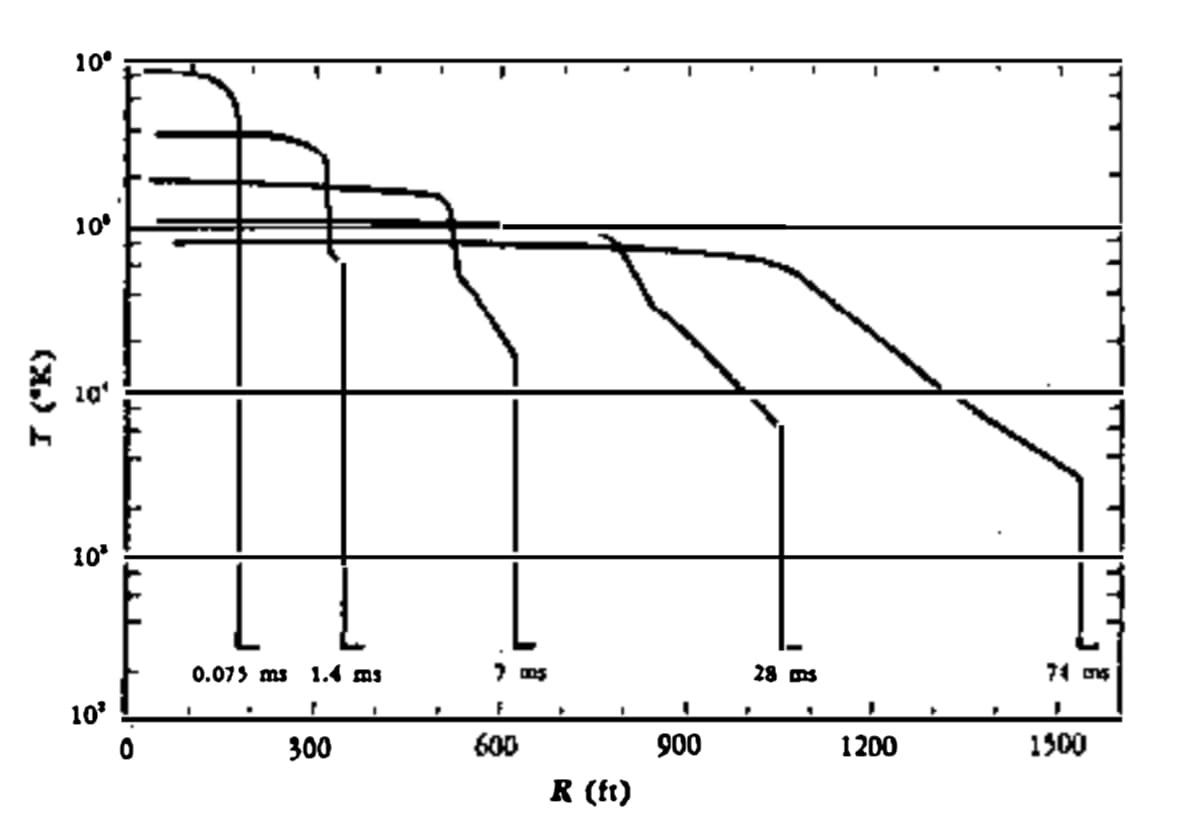
\includegraphics[width=0.5\linewidth]{img/img1}
	\caption{Temperaturen in Abhänigkeit von der Entfernung für verschiedene kurze Zeiten nach einer Explosion der Energie $\SI{1}{\mega \tnt}$.\cite{AnnuRev18_1}}
\end{figure}
\pdfnote{5555°C Siedepunkt Wolfram}
\end{frame}
\begin{frame}{Temperaturverlauf 2}
	\begin{figure}
		\centering
		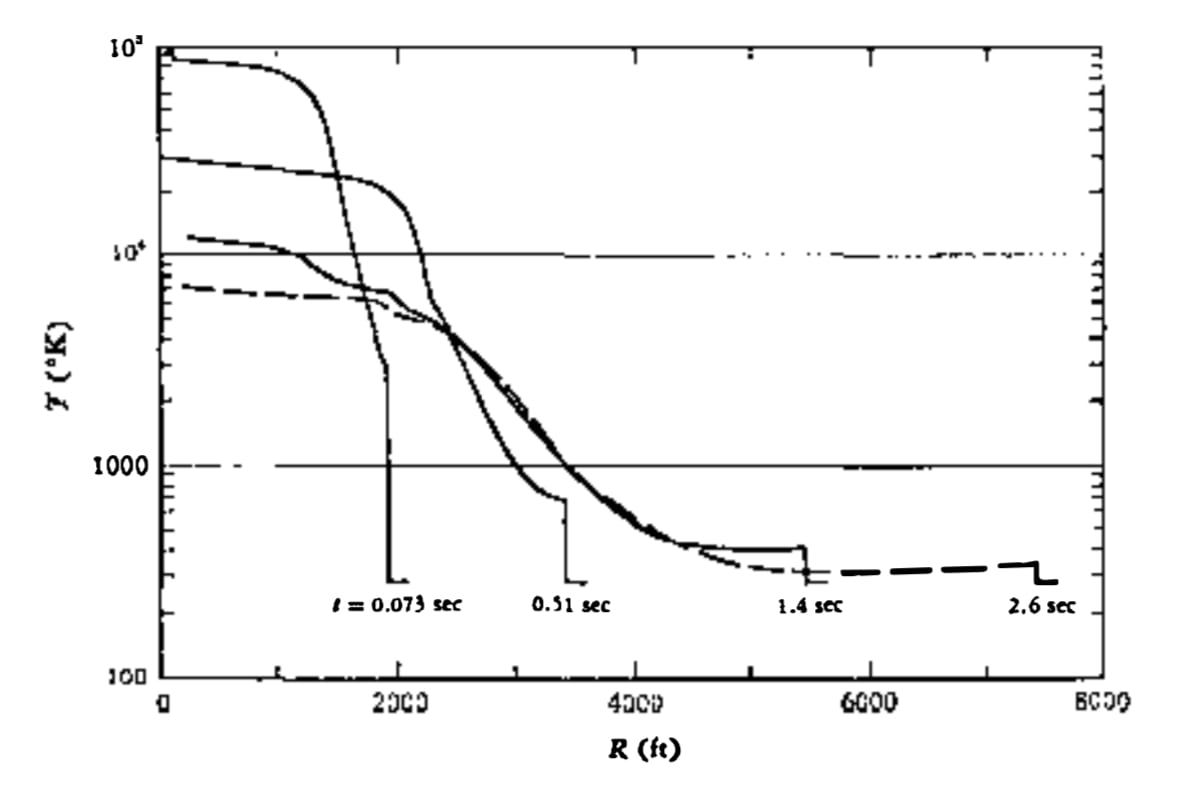
\includegraphics[width=0.5\linewidth]{img/img3.jpg}
		\caption{Temperaturen in Abhängigkeit von der Entfernung für verschiedene längere Zeiten nach einer Explosion der Energie $\SI{1}{\mega \tnt}$.\cite{AnnuRev18_1}}
	\end{figure}
	\pdfnote{1400°C Schmelzpunkt von Stahl}
\end{frame}
\begin{frame}{Druckwelle 1}
	\begin{figure}
		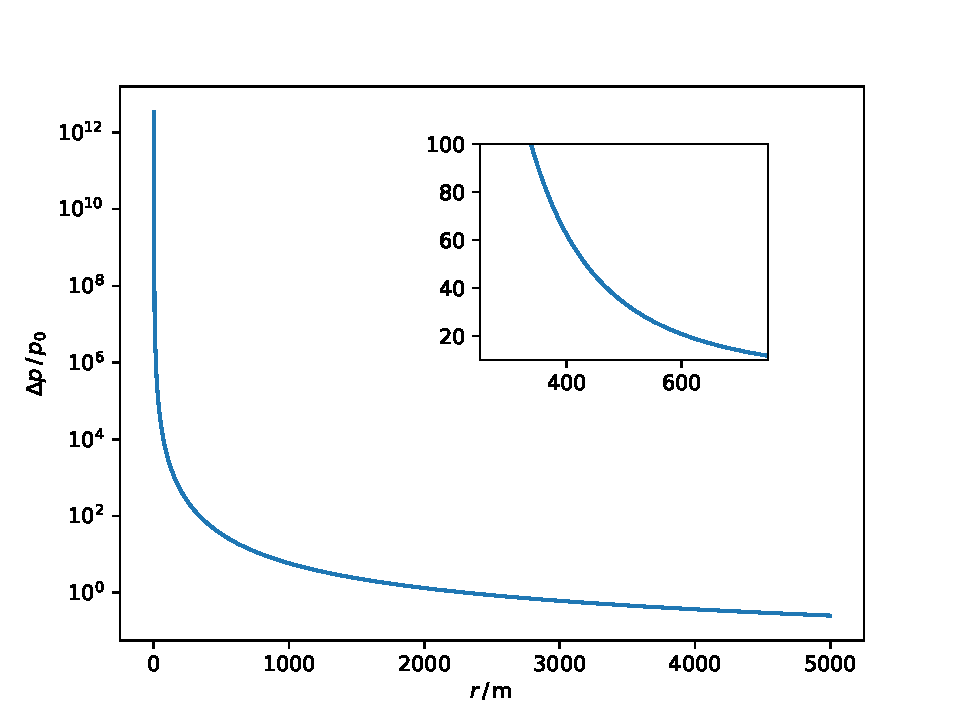
\includegraphics[width=0.5\linewidth]{img/over.pdf}
		\caption{Spitzendruck einer $\SI{1}{\mega \tnt}$ Explosion in Abhänigkeit der Entfernung.}
	\end{figure}
\end{frame}
\begin{frame}{Druckwelle 2}
\begin{figure}
	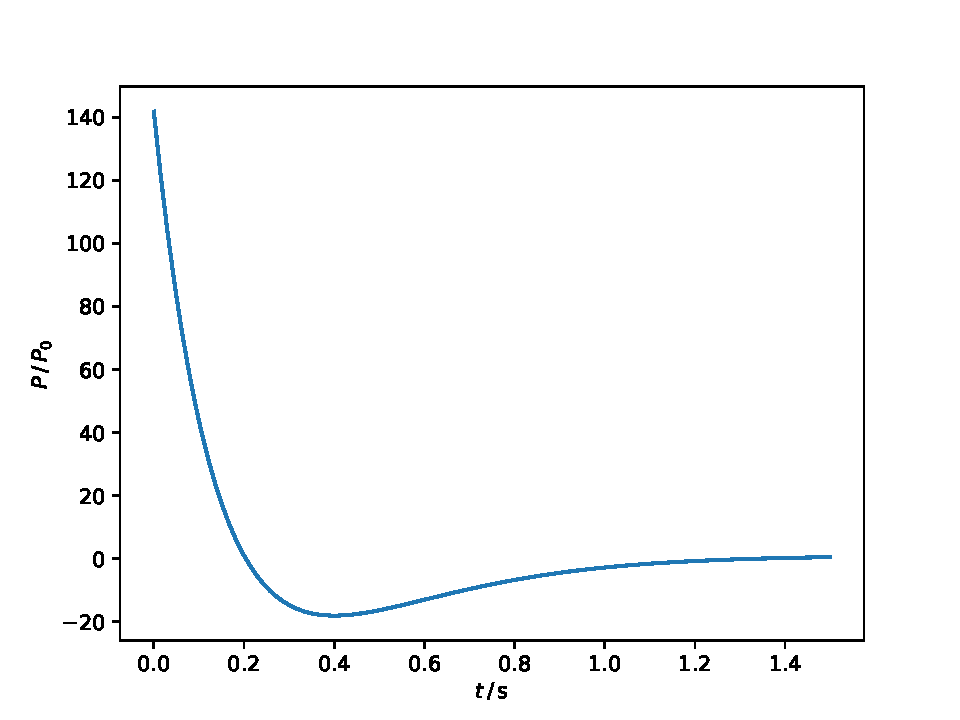
\includegraphics[width=0.5\linewidth]{img/fried.pdf}
	\caption{Zeitlicher Verlauf der Drucks einer $\SI{1}{\mega \tnt}$ Explosion in $\SI{300}{\meter}$ Entfernung.}
\end{figure}
\pdfnote{nach Friedlander Formel}
\end{frame}
\begin{frame}{Druckverlauf}
	\begin{figure}
		\centering
		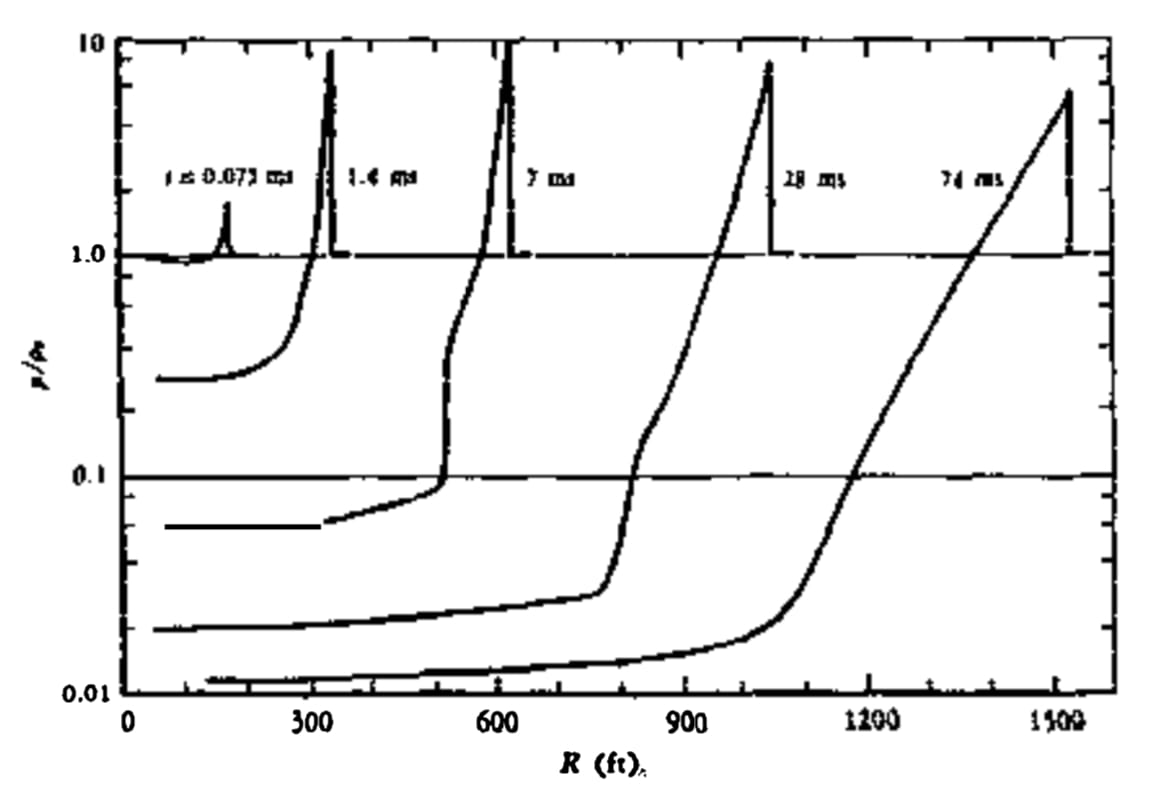
\includegraphics[width=0.5\linewidth]{img/img2.jpg}
		\caption{Luftdruck in Abhängigkeit der Entfernung für verschiedene Zeiten nach einer Explosion der Energie $\SI{1}{\mega \tnt}$.\cite{AnnuRev18_1}}
	\end{figure}
	\pdfnote{50Mt TNT Zar-Bombe}
\end{frame}
\begin{frame}{Übersicht}
	\begin{itemize}
		\item starke Überdruckwelle, gefolgt von ebenfalls großer Unterdruckwelle
		\item gigantische Hitzeentwicklung
		\item vierstellige Temperaturen in Kilometern Entfernungen
	\end{itemize}
\end{frame}
\begin{frame}{Beispiel}
	\begin{block}{Video}
		\begin{figure}
			\centering
			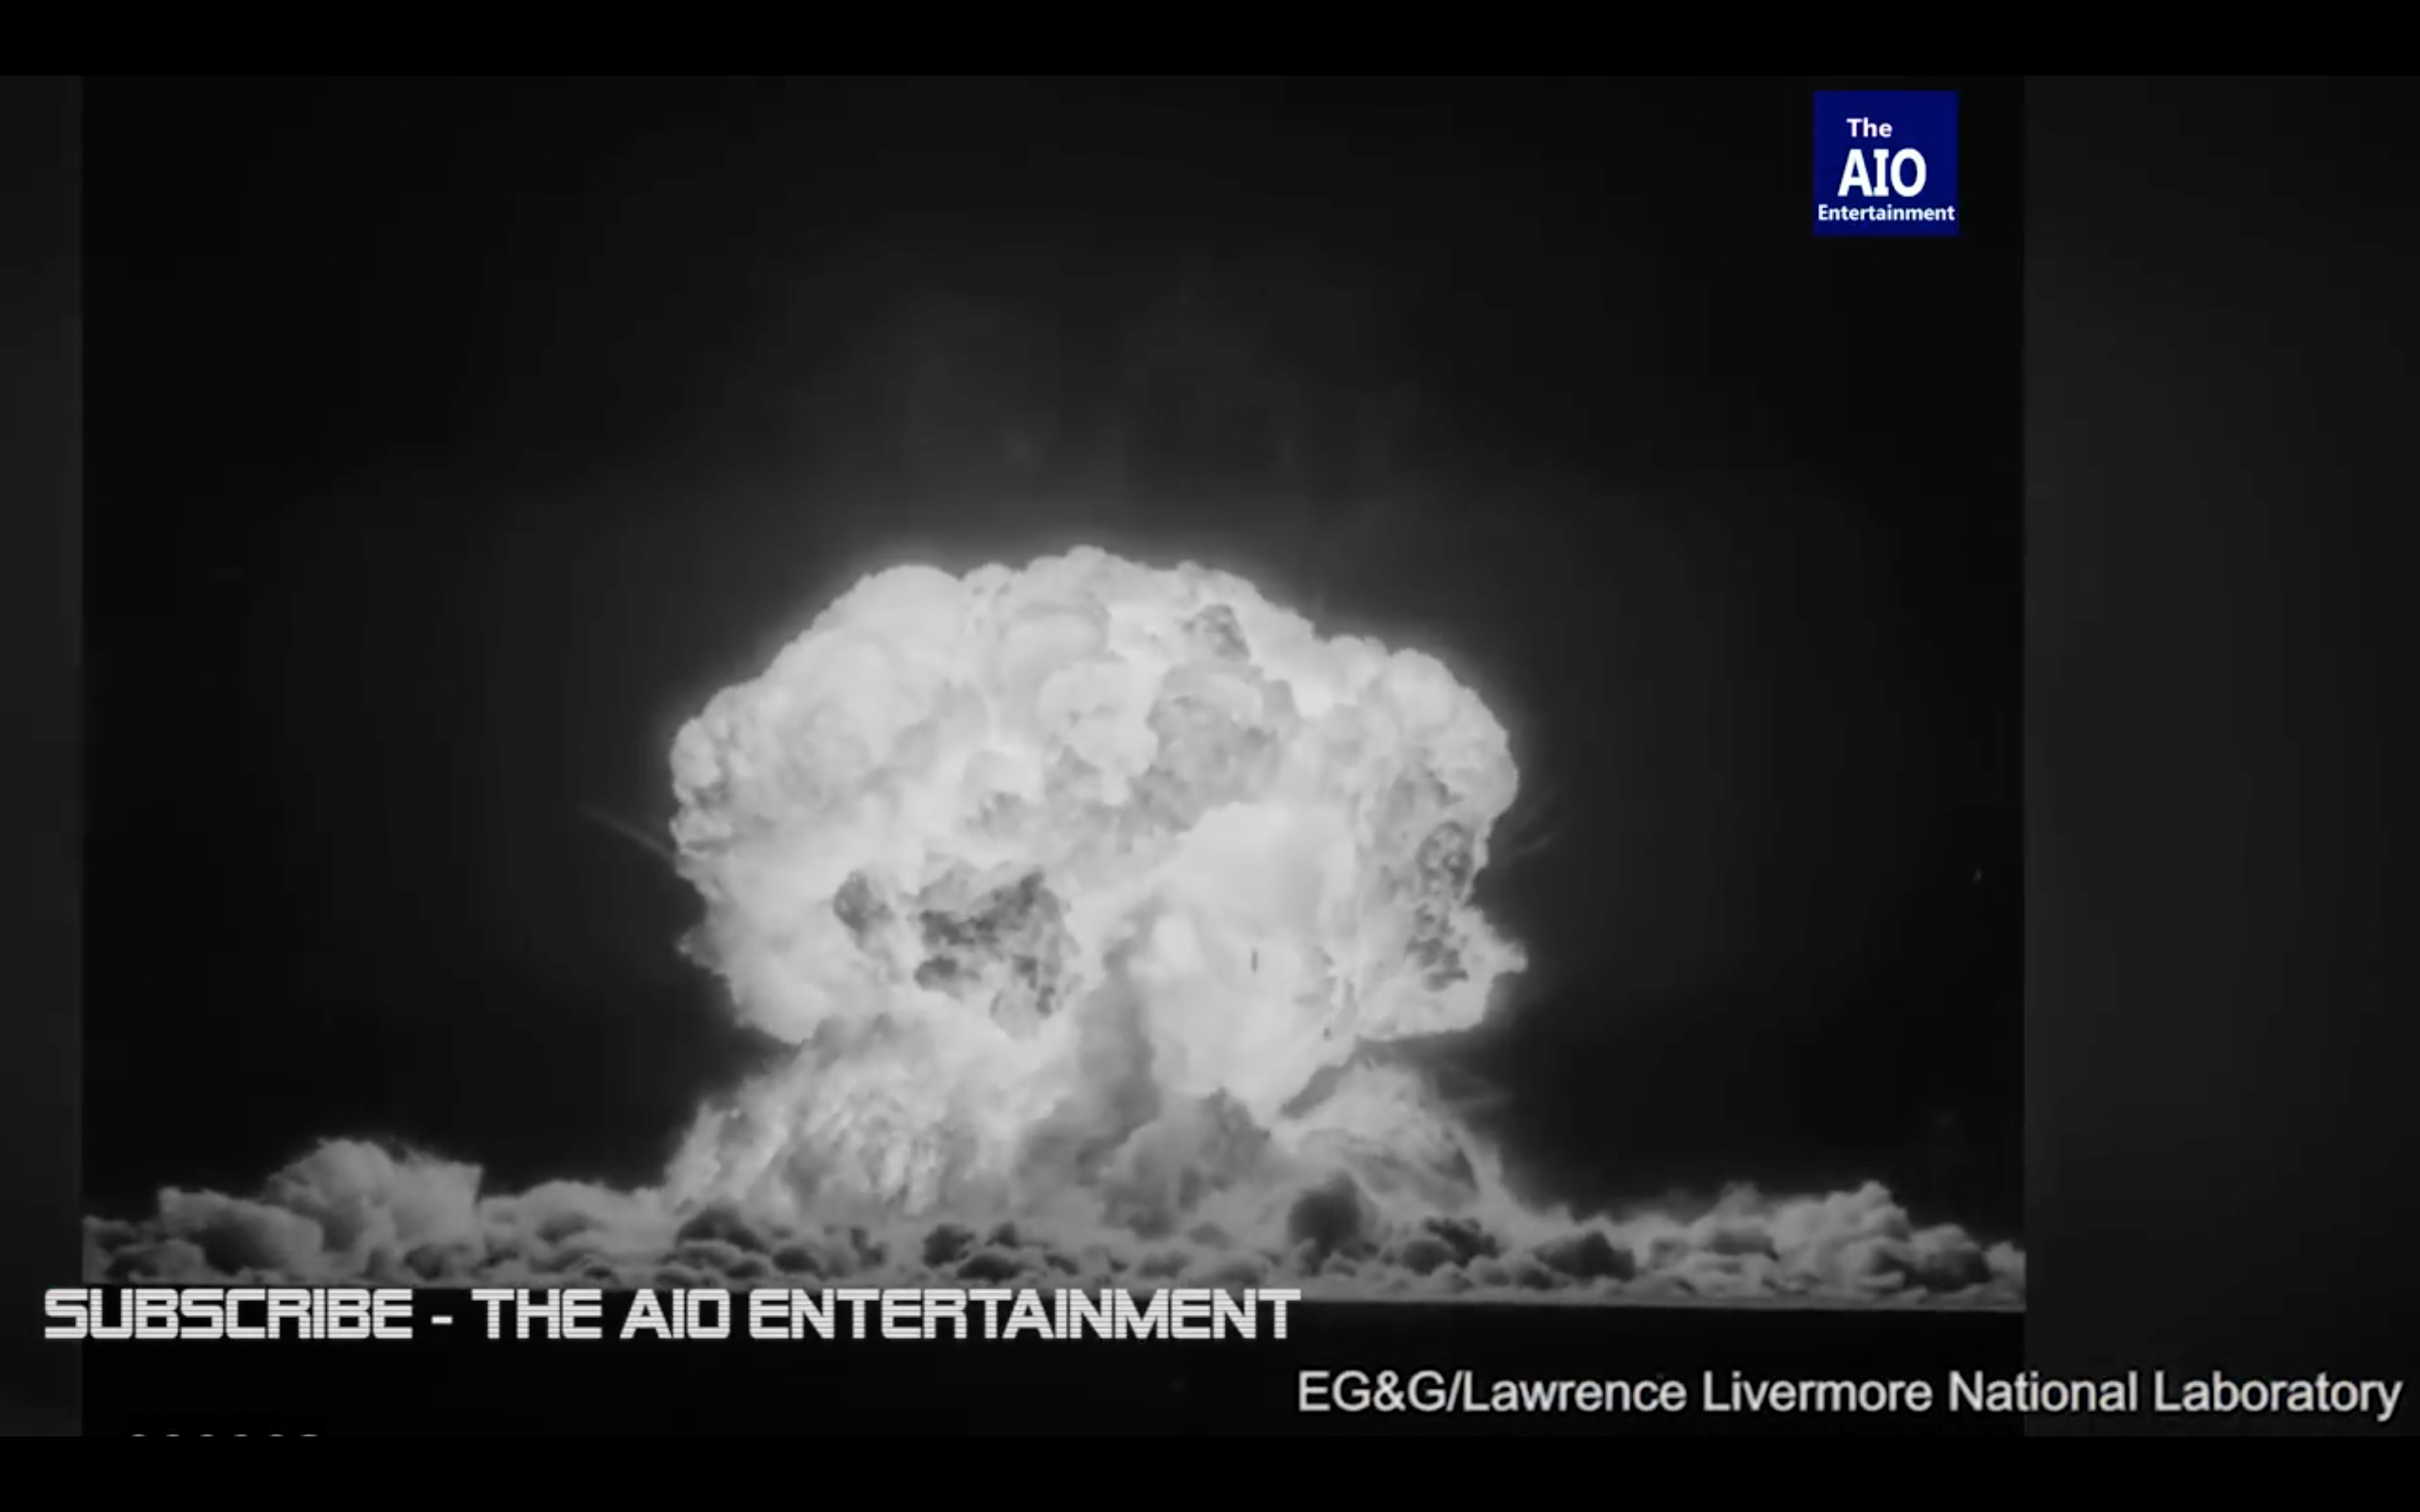
\includegraphics[width=0.5\textwidth]{img/us_nuclear_test.jpg}
			\caption{Ausschnitt von \href{https://www.youtube.com/watch?v=E3xnUE8KzwM}{Declassified US nuclear bomb test footage} }
		\end{figure}
	\end{block}
\end{frame}
